\chapter{Конструкторский раздел}

\section{Архитектура Web-приложения}
Будет использоваться популярный шаблон проектирования Web приложений Model-View-Controller. Этот шаблон разделяет работу веб-приложения на три отдельные функциональные роли: модель данных (model), пользовательский интерфейс (view) и управляющую логику (controller). Таким образом, изменения, вносимые в один из компонентов, оказывают минимально возможное воздействие на другие компоненты.

В данном паттерне модель не зависит от представления или управляющей логики, что делает возможным проектирование модели как независимого компонента и, например, создавать несколько представлений для одной модели.

Фактически, связка вида и контроллера является интерфейсом пользователя. Причем, если компоненты вида обычно можно повторно использовать в других компонентах системы, то контроллер часто является специфичным для данного конкретного случая.

Модель не зависит ни от вида, ни от контроллера, что позволяет одновременно строить различные интерфейсы пользователя для взаимодействия с одной и той же моделью данных.

\begin{figure}[h]
  \centering
  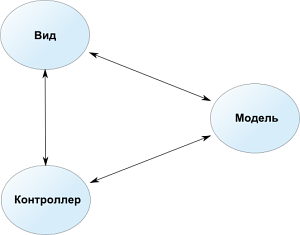
\includegraphics[width=\textwidth]{mvc_schema.png}
  \caption{ Структура шаблона “Модель – Вид – Контроллер”.}
\end{figure}

\subsection{Вид}

\textbf{Вид (View)} представляет собой компонент системы для отображения состояния модели в понятном человеку представлении. Это могут быть диалоги, формы и другие визуальные и не визуальные (например, синтезатор речи) средства взаимодействия человека с системой. Вид не изменяет данные напрямую (режим только чтение), данные изменяются при помощи контроллера.

В данной работе вид будет представлен страницами:

\begin{enumerate}
\item add-book (добавление книги)
\item authorization (авторизация)
\item create-task (создание задачи)
\item edit-profile (редактирование профиля)
\item index (главная страница)
\item list-books (список книг)
\item list-my-tasks (список задач пользователя)
\item list-search-tasks (результат поиска по задачам)
\item list-tasks (список задач пользователей)
\item registration (регистрация)
\end{enumerate}

\subsection{Контроллеры}

\textbf{Контроллер (Controller)} является средством, при помощи которого пользователи взаимодействуют с системой. Это может быть клавиатура, мышь и т. д. А также является управляющим элементом для обмена данными и сообщениями между видом и моделью.

В данной работе контроллеры представлены классами в коде, которые обрабатывают get и post запросы из страниц вида.

\begin{enumerate}
\item AddBookServlet
	\begin{itemize} 
	\item Post запрос:	
	Добавление книги в БД.
	\end{itemize}
\item AuthorizationServlet
	\begin{itemize} 
	\item Post запрос:
	Авторизация пользователя.
	\end{itemize}
\item CategoryServlet
	\begin{itemize} 
	\item Post запрос:
	Установка категории и вывод списка задач этой категории.
	\end{itemize}
\item CloseTaskServlet
	\begin{itemize} 
	\item Post запрос:
	Закрытие задачи
	\end{itemize}
\item CreateTaskServlet
	\begin{itemize} 
	\item Post запрос:
	Добавление задачи в БД.
	\end{itemize}
\item EditProfileServlet
	\begin{itemize} 
	\item Post запрос:
	Изменение данных пользователя.
	\end{itemize}
\item LibraryServlet
	\begin{itemize} 
	\item Post запрос:
	Установка категории и вывод списка книг этой категории.
	\end{itemize}
\item LikeBookServlet
	\begin{itemize} 
	\item Post запрос:
	Оценка книги.
	\end{itemize}
\item LikeWantToHelpServlet
	\begin{itemize} 
	\item Post запрос:
	Оценка запроса.
	\end{itemize}
\item RegistrationServlet
	\begin{itemize} 
	\item Post запрос:
	Регистрация пользователя.
	\end{itemize}
\item LogoutServlet
	\begin{itemize} 
	\item Get запрос:
	Выход авторизованного пользователя.
	\end{itemize}
\item SearchServlet
	\begin{itemize} 
	\item Post запрос:
	Текстовый поиск по задачам.
	\end{itemize}
\item WantToHelpServlet
	\begin{itemize} 
	\item Post запрос:
	Добавление заявки на помощь.
	\end{itemize}

\end{enumerate}

\subsection{Модель}

\textbf{Модель (Model)} представляет собой данные, с которыми оперирует приложение. Это могут быть как данные базы данных, так и любая другая структура данных, описывающая некоторые объекты системы и их состояние.

Различают пассивный и активный режимы работы с моделью данных.

При \textbf{пассивном режиме} данные на клиентской стороне перечитываются при выполнении некоторых действий пользователя, например, запроса на вывод информации об объектах.

При \textbf{активном режиме} вводятся дополнительные обработчики и слушатели сообщений, которые посылают компонентам уровня представления сообщения о том, что данные модели были изменены и требуется обновление данных на стороне клиента “View”.

В данной работе используется пассивный режим работы с моделью данных.

Модели представлены классами:
\begin{enumerate}
\item Book
\item Category
\item LikeBook
\item Member
\item Task
\item University
\item WantToHelp
\end{enumerate}

Использование реляционной базы данных для хранения объектно-ориентированных данных приводит к семантическому разрыву, заставляя программистов писать программное обеспечение, которое должно уметь, как обрабатывать данные в объектно-ориентированном виде, так и уметь сохранить эти данные в реляционной форме. Эта постоянная необходимость в преобразовании между двумя разными формами данных не только сильно снижает производительность, но и создает трудности для программистов, так как обе формы данных накладывают ограничения друг на друга.
Разработано множество пакетов, устраняющих необходимость в преобразовании объектов для хранения в реляционных базах данных.

Некоторые пакеты решают эту проблему, предоставляя библиотеки классов, способных выполнять такие преобразования автоматически. Имея список таблиц в базе данных и объектов в программе, они автоматически преобразуют запросы из одного вида в другой.

С точки зрения программиста система должна выглядеть как постоянное хранилище объектов. Он может просто создавать объекты и работать с ними как обычно, а они автоматически будут сохраняться в реляционной базе данных.

\textbf{ORM (англ. Object-Relational Mapping, рус. объектно-реляционное отображение)} — технология программирования, которая связывает базы данных с концепциями объектно-ориентированных языков программирования, избавляет программиста от написания большого количества кода, часто однообразного и подверженного ошибкам, тем самым значительно повышая скорость разработки. Кроме того, большинство современных реализаций ORM позволяют программисту при необходимости самому жёстко задать код SQL-запросов, который будет использоваться при тех или иных действиях (сохранение в базу данных, загрузка, поиск и т. д.) с постоянным объектом.

На практике всё не так просто и очевидно. Все системы ORM обычно проявляют себя в том или ином виде, уменьшая в некотором роде возможность игнорирования базы данных. Более того, слой транзакций может быть медленным и неэффективным (особенно в терминах сгенерированного SQL). Все это может привести к тому, что программы будут работать медленнее и использовать больше памяти, чем программы, написанные «вручную».

На данном этапе разработки системы принято решение использовать технологию ORM.


